\chapter{Diseño e Implementación} % Main chapter title

\label{Chapter3} % Change X to a consecutive number; for referencing this chapter elsewhere, use \ref{ChapterX}
\definecolor{mygreen}{rgb}{0,0.6,0}
\definecolor{mygray}{rgb}{0.5,0.5,0.5}
\definecolor{mymauve}{rgb}{0.58,0,0.82}

\lstset{ %
  backgroundcolor=\color{white},   % choose the background color; you must add \usepackage{color} or \usepackage{xcolor}
  basicstyle=\footnotesize,        % the size of the fonts that are used for the code
  breakatwhitespace=false,         % sets if automatic breaks should only happen at whitespace
  breaklines=true,                 % sets automatic line breaking
  captionpos=b,                    % sets the caption-position to bottom
  commentstyle=\color{mygreen},    % comment style
  deletekeywords={...},            % if you want to delete keywords from the given language
  %escapeinside={\%*}{*)},          % if you want to add LaTeX within your code
  %extendedchars=true,              % lets you use non-ASCII characters; for 8-bits encodings only, does not work with UTF-8
  %frame=single,	                   % adds a frame around the code
  keepspaces=true,                 % keeps spaces in text, useful for keeping indentation of code (possibly needs columns=flexible)
  keywordstyle=\color{blue},       % keyword style
  language=[ANSI]C,					% the language of the code
  %otherkeywords={*,...},           % if you want to add more keywords to the set
  numbers=left,                    % where to put the line-numbers; possible values are (none, left, right)
  numbersep=5pt,                   % how far the line-numbers are from the code
  numberstyle=\tiny\color{mygray}, % the style that is used for the line-numbers
  rulecolor=\color{black},         % if not set, the frame-color may be changed on line-breaks within not-black text (e.g. comments (green here))
  showspaces=false,                % show spaces everywhere adding particular underscores; it overrides 'showstringspaces'
  showstringspaces=false,          % underline spaces within strings only
  showtabs=false,                  % show tabs within strings adding particular underscores
  stepnumber=1,                    % the step between two line-numbers. If it's 1, each line will be numbered
  stringstyle=\color{mymauve},     % string literal style
  tabsize=2,	                   % sets default tabsize to 2 spaces
  title=\lstname,                   % show the filename of files included with \lstinputlisting; also try caption instead of title
  morecomment=[s]{/*}{*/}%
}

% -------------------------------------

En este capítulo se muestra todo el proceso de desarrollo del dispositivo, tanto el firmware como hardware. Se explica según el orden del modelo en V aplicado.

% --------------------------------------

\section{Modelo de desarrollo}


El proceso de desarrollo elegido es el modelo en V


\section{Implementación del sistema}

El equipo digitaliza señales analogicas provenientes de dos sensores de presión intrarterial del tipo strain-gauge y almacena las señales por períodos prolongados de alrededor de 24 hs. Estas señales adquiridas se guardan en una memoria de tipo flash (memoria SD), y pueden descargarse a una PC a través de una interfaz USB. Desde la PC se accede a los archivos guardados como un medio de almacenamiento masivo, y se pueden visualizar en cualquier software que permita procesar un archivo de tipo ".csv".

Previo a cada experiencia, el operador configura el equipo desde una terminal Bluetooth, como una tablet o una PC, a través de un protocolo de comunicación muy sencillo que se desarrolló para este proyecto. A través de esta interfaz se configuran parámetros como la frecuencia de muestreo, la cantidad de canales a usar, ganancia del amplificador programable, seteo de hora y fecha, y finalmente se da inicio a la medición. 

El equipo consiste en un sistema embebido portátil basado en un microcontrolador ARM de 32 bits, Cortex M3: LPC1769, un conversor analógico digital de alta resolución (ADS1292), módulos de comunicación (serie, BLE, USB), almacenamiento masivo (SD) y módulo de regulación de energía y carga de batería. Puede verse un diagrama en bloques en la Figura \ref{fig:diag_bloques} . Para este proyecto se utilizaron en forma intensiva la gran mayoría de los contenidos y herramientas vistas durante el Carrera de Especialización en Sistemas Embebidos (CESE). Se utilizaron técnicas de Gestión de Proyectos, documentación manual y automática del trabajo, sistema de versionado de software y hardware. En cuanto a lo técnico se emplearon conocimientos específicos sobre arquitectura del microcontrolador, modelos de programación, sistema operativo de tiempo real freeRTOS, protocolos de comunicación (BLE, SPI, USB, y de alto nivel), testing unitarios, etc.


\begin{figure}[!htbp]
	\centering
	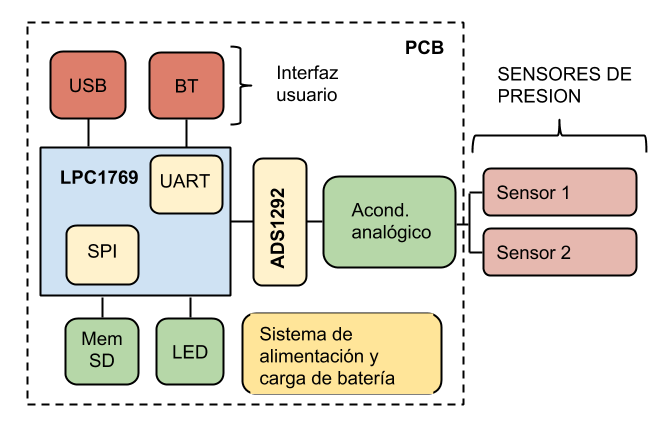
\includegraphics[width=\textwidth]{./Figures/diag_bloques.png}
	\caption{Diagrama en bloques del equipo.}
	\label{fig:diag_bloques}
\end{figure}


%----------------------------------------------------------------------------------------
%	SECTION 1
%----------------------------------------------------------------------------------------
\section{Análisis del software}
 
En esta sección se resaltan los problemas encontrados, los criterios utilizados y la justificación de las decisiones que se hayan tomado.

Se puede agregar código o pseudocódigo dentro de un entorno lstlisting con el siguiente código:

\begin{verbatim}
\begin{lstlisting] [caption= "un epígrafe descriptivo"]

	las líneas de código irían aquí...
	
\end{lstlisting}
\end{verbatim}

A modo de ejemplo:

\begin{lstlisting}[caption=Pseudocódigo del lazo principal de control.]  % Start your code-block

#define MAX_SENSOR_NUMBER 3
#define MAX_ALARM_NUMBER  6
#define MAX_ACTUATOR_NUMBER 6

uint32_t sensorValue[MAX_SENSOR_NUMBER];		
FunctionalState alarmControl[MAX_ALARM_NUMBER];	//ENABLE or DISABLE
state_t alarmState[MAX_ALARM_NUMBER];						//ON or OFF
state_t actuatorState[MAX_ACTUATOR_NUMBER];			//ON or OFF

void vControl() {

	initGlobalVariables();
	
	period = 500 ms;
		
	while(1) {

		ticks = xTaskGetTickCount();
		
		updateSensors();
		
		updateAlarms();
		
		controlActuators();
		
		vTaskDelayUntil(&ticks, period);
	}
}
\end{lstlisting}



